\documentclass{journal}

\title{On Goto Killing You in Your Sleep}
\author{1707981}
\date{\today}

\usepackage{graphicx}
\usepackage{xcolor}
\usepackage{listings}

\definecolor{codebackground}{rgb}{0.8, 0.8, 0.8}

\lstdefinestyle{genius}{
	tabsize = 2,
	basicstyle = \tiny,
    captionpos = b,
    backgroundcolor = \color{codebackground},
    breaklines = true,
    frame = single
}

\lstset{style=genius}

\begin{document}
\maketitle

% Basic competency: 40% 1 peer review, viva discussion, citations appropriate, academically integral
% Breadth of reading: 10% -- read lots of articles, 16 of them!
% Depth of insight: 15% Significant insight demonstrated. Discussion is anlytical and evaluative in nature
% Specificability, verifiablility and accuracy of claims: 10%, all claims have a clear source of evidence. Almost no errors/misinterpretations.
% Synthesis: 15%, Info from multiple sources synthesised into a strongly cohesive whole. Connections are analytical and evaluative.
% Spelling & grammar: 5%
% Structure: 5%
% \textbf \textit \underline

% https://dl-acm-org.ezproxy.falmouth.ac.uk/citation.cfm?id=363570&CFID=828610973&CFTOKEN=85313317
% response to Dijkstra: "How many poor, innocent, novice programmers will feel guilty when their sinful use of go to is flailed in this letter?"

% The humble programmer
% In his marriage certificate Dijkstra is a 'theoretical physicist'

\section{``Introduction'':;}
In March 1968, the notorious `Go to statement considered harmful' \cite{goto} letter was penned by Edsger W. Dijkstra, an influential pioneer of computer science during its early days. He helped push a revolution for structured programming \cite{structured}, effectively sparking exhaustive efforts to deprecate the goto statement \cite{revolution1, againstgoto} across the community. His paper can be summarised as a criticism that using goto statements causes the flow of the program's execution to diverge greatly from the flow of text, by allowing the process to jump to various areas in code in an unstructured manner, with no obvious indicators from where it came. Due to the compromise in human readability he proposed that the use of goto statements be avoided outside machine level code.

Dijkstra's words were bold in their criticism of what was once common practice [CITE]. While his motivation was apparently just a negative correlation between a programmer's skill quality and the number of goto statements in their code \cite{goto, humanprogramming}, the observant would recognise Dijkstra as the creator of the popular collision-avoiding pathfinding algorithm of the same name \cite{pathfinding}, and could conclude that his objection to the goto statement was motivated because the ability to `go to' anywhere is far too easy. Dijkstra's subsequent collision-free descent into madness, which pulled many programmers and academics along with him in the cold, harmful grasps of the ``considered harmful'' phenomenon, in his ever deepening existential crisis illustrating how virtually everything in programming is flawed in some way as our souls are meanwhile sold to the terrible programmers in the megacorporations of tomorrow \cite{truths}, began here.

For an illustration of Dijkstra's pathfinding algorithm, \textbf{go to ``Pathfinding''}.

Else for the next section of this essay, \textbf{go to ``To Pascal''}

\setcounter{section}{4}
\section{``Conclusions'':;}
Today it is truly a wonder whether the goto statement has a right to exist, similar to the enigma of whether programmers have a right to exist with it. This appears to be why the goto statement is still fully intact today; while perhaps only 10\% of uses \cite{github} go backwards, nobody can truly predict how the volatile community of programmers would react to a stripped or modified feature. Thus it seems that goto is here to stay until the next revolutionary programming language comes along. Until then, we work our traditional programming languages standing at around 30 to 50 years old [CITE], hardly escaping the goto controversy in their days, as if in an infinite loop. While a goto-free world may be in our future, we hesitate to goto that place anytime soon.

\textbf{Go to ``Introduction''}

\setcounter{section}{3}
\section{``Goto in Practice'':;}
To see whether a backwards goto statement is useful, it is worth exploring where goto is typically used. An extensive study \cite{gotostudy} of the world's largest open code repository \cite{github}, GitHub, found that most goto statements in modern C code are used for error handling. This is usually characterised by a function, sometimes loading various error-dependent resources; followed by a function ending, returning success; then followed by an `error:' label of such, beneath which any loaded resources are freed before returning. This is popular, but does not necessitate a backwards-capable goto statement as the error condition is usually placed at the end of the function \cite{gotostudy}.

\begin{lstlisting}[language=C,caption={An example of goto used for error handling (C)}]
bool DeliberatelyCorruptThisEssay() {
	FILE *file1 = NULL, *file2 = NULL, *file3 = NULL;
	
	file1 = fopen("essay.tex", "w");
	[...] // do malicious stuff
	file2 = fopen("excuse_for_no_submission.txt", "w")
	[...] // do suspicious stuff
	if (!file2)
		goto Error; // don't worry I got this brah
	file3 = fopen("allies_in_crime.txt", "w");
	if (!file3)
		goto Error; // goto power corruption intensifies
	[...] // do duplicitous stuff
	Success:
	return true; // essay corrupted and defense constructed
	Error:
	[...] // cleanup for any number of unclosed files
	return false; // uh oh, guess we need to hand this in
}
\end{lstlisting}

The study similarly concluded that 90\% of goto uses were forward-only, and believed to be used for reasonable purposes. It is likely these are the reasons goto still exists: it has fairly common uses; and in retrospect, the primary concern was never the statement itself, but its habitual use -- such was the first inspiration within Dijkstra's paper \cite{goto}. It can thus be safely assumed that the programmer does in fact have control of the devil's powers after all, and that goto can be used for good; and it is perhaps us who are evil. As such, it is amusing that the statement itself has gained so much criticism compared to those who abuse it--and perhaps Wirth deserves more credit for actively promoting structured habits with Pascal \cite{pascal}, \cite{pascalrecollections}.

\textbf{Go to ``Conclusions''}

\setcounter{section}{1}
\section{``To Pascal'':;}
Dijkstra's disdain was not unique. His paper itself found inspiration from the words of N. Wirth, who with C. A. R. Hoare \cite{algolwirth} advised the demotion of labels and goto statements whilst proposing changes to the ALGOL language in 1965, with a similar rationale that the structure of a program should be tree-oriented. In their proposal, `goto' would be stripped of all complexities, leaving no more than a functional jump statement should the ability to jump anywhere in code ever be needed.

As an interesting side remark, this required a restructuring of ALGOL's switch statement, to be replaced by the case statement \cite{algolwirth}. The original switch statement was considerably different to its modern incarnation. For an example, \textbf{go to ``Switch statements''}.

In fact compared to Dijkstra, it is arguable that it was Wirth who took the more active role in demoting goto in favour of structured programming. When he and his team's proposals for ALGOL were rejected in favour of a more complex overhaul (to become ALGOL 68) \cite{pascalrecollections}, Wirth began work on ALGOL W, whilst the Working Group created ALGOL 68. Soon after, ALGOL 68 failed, creating a new hole in the market through which Wirth threaded in 1970 with his new language, Pascal \cite{pascalrecollections}.

Wirth's goal in creating Pascal was to advance programming languages -- despite the widespread application of far more popular, yet stagnated ones -- resulting in a language with improved structure and an easier learning curve \cite{pascal}. He focussed on encouraging structured programming, explained in great detail in a book partly authored by Dijkstra himself \cite{structured}, wherein code is written in a tree structure, flowing downward roughly proportionally to the internal process he originally \cite{goto} described.

Yet contrary to all those developments, for some reason, goto statements still existed, even implemented into Pascal itself \cite{pascal}.

\textbf{Go to ``Prevalence of the goto feature''}

\setcounter{section}{2}
\section{``Prevalence of the goto feature'':;}
Like a forbidden fruit or a cigarette box, goto somehow still exists in programming languages, with a large `DO NOT USE' written on its packet. In fact, one of the most popular programming languages of today, C, has a functional goto statement, described by D. Ritchie as infinitely abusable and unnecessary \cite{cprogramming} as he gleefully implemented it into the compiler. It calls to question, if goto were truly harmful, why is it still included in modern programming languages? Even Microsoft's modern interpretation of C++, C\#, features a version of goto that is in fact expanded to also support switch labels \cite{csharp}. Why plant evil in the garden and call it a weed?

On first glance, it appears that `goto' is included just to ensure the feature is available for backward compatibility. However, the extreme unpopularity of the goto statement (\cite{goto}, \cite{againstgoto}) creates strong reasoning to remove it. As it stands, programmers are likely to avoid using it purely for sentimental reasons--sometimes at the expense of a larger line count and computation time \cite{caseforgoto}, which is one consideration for its raison d'être.

Indeed, there are valid uses for goto, some of which were illustrated in F. Rubin's letter \cite{gotoodeep}, disputing Dijkstra's one (and considered `disappointing' \cite{disappointing}). A popular use is when breaking out of deeply embedded loops under a particular condition \cite{gotoodeep}. This is in fact also described in the C programming book itself \cite{cprogramming}, raising the question; hypothetically speaking, is there not an alternative way to achieve this? When one needs to jump to a different area of code, namely a different scope, a jumping statement seems like a reasonable solution. And in order to break out into a shallower scope, would it not be best practice to refer to it by a name? Is that not a goto statement?

\begin{lstlisting}[language=C,caption={An example of goto used for breaking loops (C)}]
void ImInTooDeep() {
	for (Friend* f = friends[0]; f < &friends[numFriends]; f++) {
		for (Friend* ff = f->friends[0]; ff < &f->friends[f->numFriends]; ff++) {
			for (Friend* fff = ff->friends[0]; fff < &ff->friends[ff->numFriends]; ff++) {
				if (fff->LikesYourPlushie())
					goto FoundSomeone; // no other way to break all loops at once
			}
		}
	}

	printf("No-one relevant to your life likes your Pikachu plushie\n");
	return; // end function here if goto not occured
	FoundSomeone:
	printf("There is a glimmer of hope. Pika!");
	return; // here returning from the Void is optional, but we'll do it for health and safety
}
\end{lstlisting}

An article by W. Wulf \cite{againstgoto} addressed one particular solution to the above problem, featured in the Bliss programming language: to include a `leave' statement to escape from a loop and jump to a label. This is potentially more readable than a goto statement, since it can only jump forward. This is a logical solution, but calls to question whether it is truly worthy to replace goto, as seemingly merely a restricted form of it? On the other hand, is there ever anything helpful about a goto statement that goes backwards?

To find out \textbf{go to ``Goto in practice;''}

\setcounter{section}{1}
\section{``Switch statements'':;}
Interestingly, the `case' statement proposal was intended to replace the `switch' statement of ALGOL 60, which at the time was effectively a declaration of an array of labels to be used with a dynamic `goto' statement \cite{algolguide}. Heavily contrast to the modern switch statement of the C family today, which essentially defines `switch' as what was Pascal's `case', and `case' as what was once the labels, except restricted within the scope of the statement. As C was inspired by the ALGOL family [CITE], it is likely that the creator of C considered this small reinterpretation as a more correct terminology.

%\begin{figure}
	%	\begin{subfigure}
	%	\end{subfigure}
%\end{figure}
% [put a figure here illustrating the different uses of the switch statement]

\textbf{Go to ``To Pascal''}

\newpage

\setcounter{section}{0}
\section{``Pathfinding'':;}
See below for an implementation of the Dijkstra's algorithm \cite{pathfinding}, remarkable in that it actually compiles. \textit{tiles} represents an 8x8 array of enumerations of either Tile::W or Tile::E where Tile::W is a wall. Visiting left and right nodes may wrap around to a different row, and exceeding the bottom left and top right corner will crash; these are special features for extra usability. It is unclear whether it actually functions, yet it does; unfortunately suggesting the computer has a better knowledge than the programmer who should be controlling it. Perhaps more goto statements would help. [?!]

\begin{figure}[h]
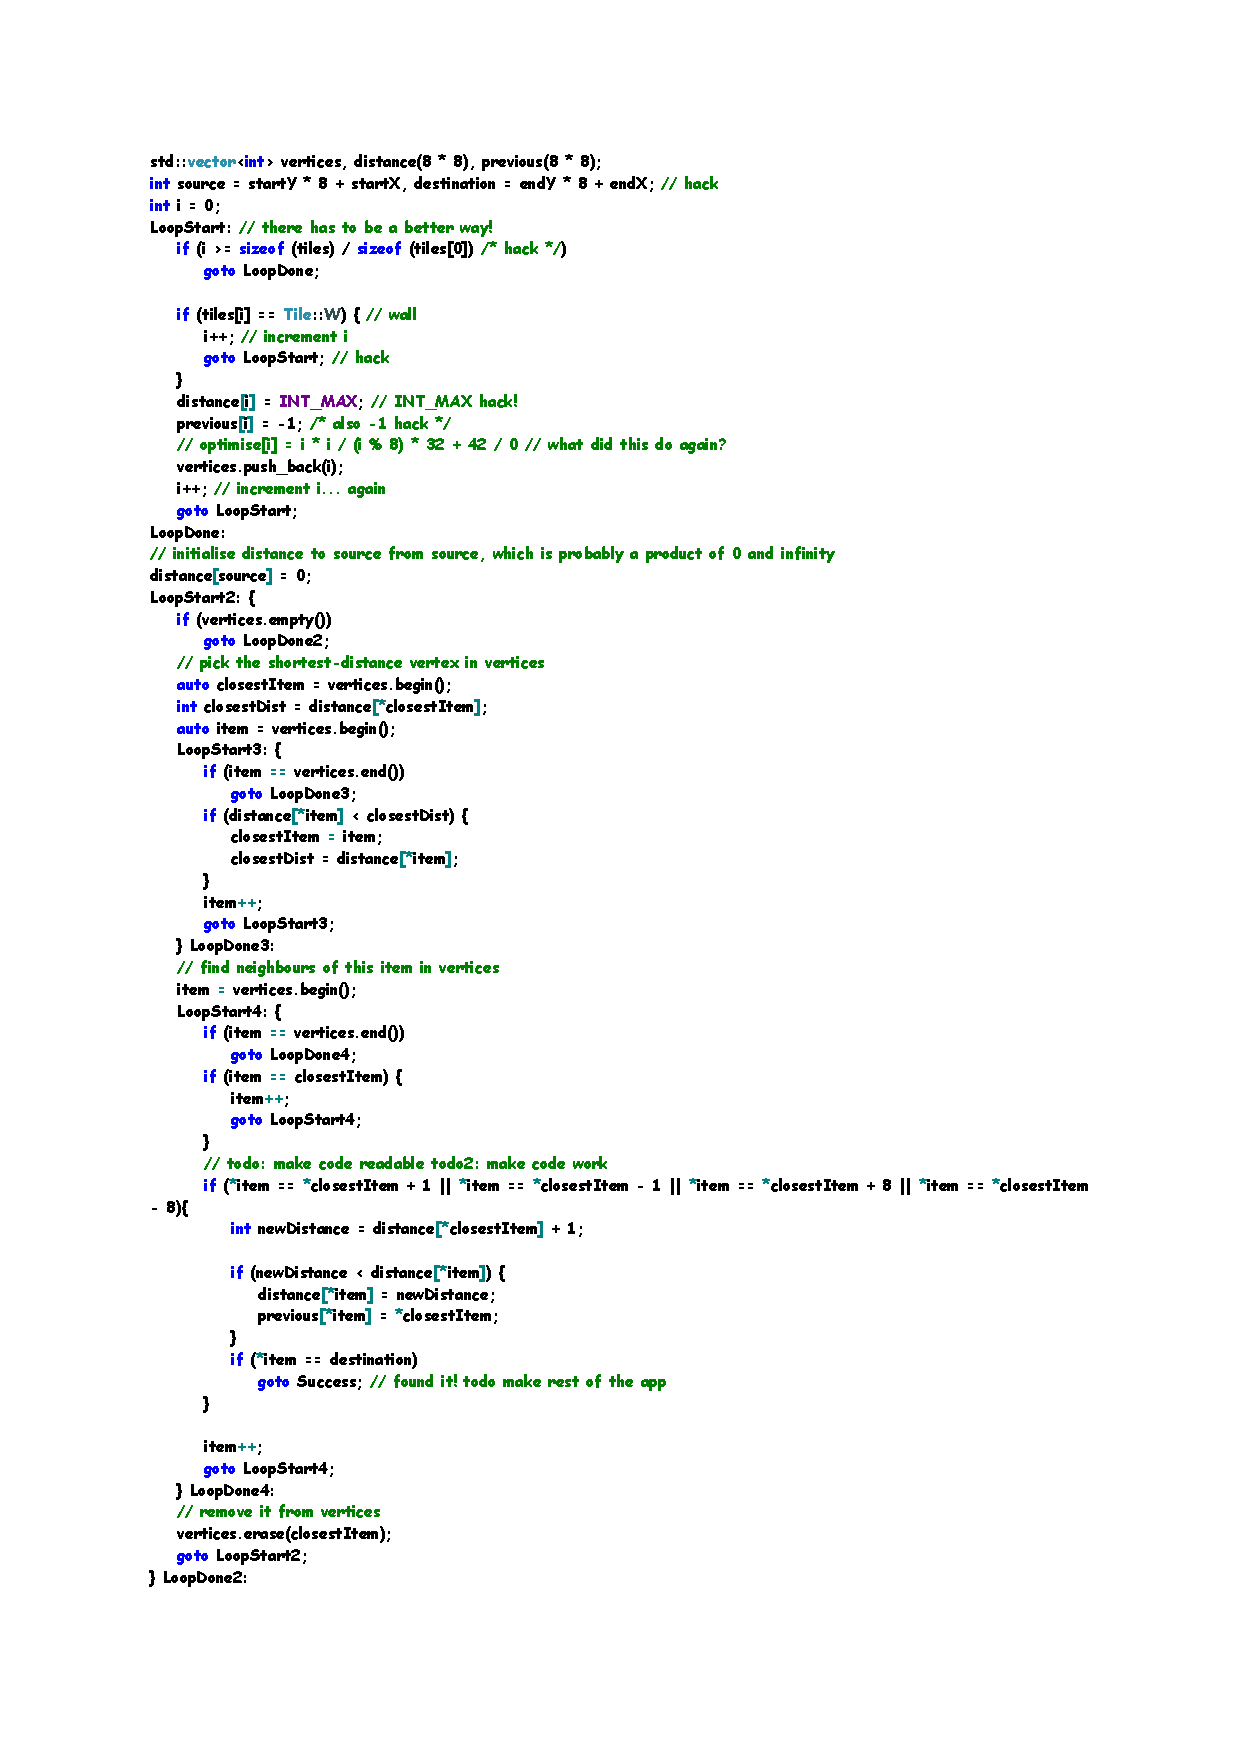
\includegraphics[width=0.8\linewidth]{Pathfinding.pdf}
\caption{A C++ implementation of Dijkstra's algorithm \cite{pathfinding} in Comic Sans}
\end{figure}

\textbf{Go to ``To Pascal''}

\bibliography{references}
\bibliographystyle{ieeetr}
\end{document}